% Provenance (never printed): BCPST year 1 geology (2021), "la carte
% geologique" (reading a map, structures, chronology), union licence
% Sciences de la Terre L1 (cartographie: strike and dip, three-point problem,
% outcrop patterns, DEM and GIS). See sources/outline_sources.md. Pilot
% chapter, 2026-10-22. The region is the series' invented Varden Hills
% (figdata/shared/region.py); every number about it is computed in
% figdata/bachelor-1/varden_maps.py or figdata/bachelor-1/v_rule.py.
\chapter{Geologische kaarten}\label{ch:b1:geological-maps}

Een geoloog trekt met een kaartbord, een notitieboekje en een kompas-kliseometer over een
reeks lage heuvels. Het meeste van de grond is gras, bos of geploegd land; gesteente is er
maar hier en daar zichtbaar, in een beekoever, een wegsnede, een rotsrichel. Uit deze
verspreide glimpen en uit de vorm van het landschap moet de geoloog zeggen welk gesteente
onder elke vierkante meter van de heuvels ligt, hoe de lagen gekanteld zijn, waar zij
gebroken zijn en in welke volgorde dit alles is gebeurd. Het resultaat is een \omterm{def:b1:geological-maps:geological-map}{geologische
kaart}: een platte tekening die een driedimensionaal gesteentelichaam codeert.
Dit hoofdstuk legt uit hoe zo'n kaart wordt gemaakt en hoe zij wordt gelezen: hoe de
oriëntatie van een vlak wordt gemeten en berekend, waarom de \omterm{def:b1:geological-maps:geological-map}{ontsluiting} van een laag de
patronen tekent die zij tekent, en hoe een kaart een geschiedenis vertelt. De voorbeelden
komen uit een verzonnen maar geologisch consistente streek, de Varden Hills, die in dit boek
steeds terugkeert.

\begin{recall}
Een topografische kaart toont het reliëf met hoogtelijnen, lijnen van gelijke hoogte; haar
schaal verbindt afstanden op de kaart met afstanden op de grond (Boek 1, klas 9). Relatieve
leeftijden volgen uit superpositie (een laag is jonger dan de lagen eronder, tenzij de reeks
omgekeerd is), uit doorsnijding (wat een gesteente doorsnijdt, is jonger dan dat gesteente)
en uit insluiting (Boek 1, klas 7). Een breuk is een scheur waarlangs de twee blokken zijn
verschoven (Boek 1, klas 7); de meetkunde van \omterm{def:b1:geological-maps:fold}{plooien} en breuken is het onderwerp van
\cref{ch:b1:faults-folds-fabrics}.
\end{recall}

\section{Een kaart is een doorsnede van drie dimensies}\label{sec:b1:geological-maps:cut}

\begin{definition}[Geologische kaart]\label{def:b1:geological-maps:geological-map}
Een \emph{geologische kaart}\index{geologische kaart} toont, op elk punt van het aardoppervlak,
de gesteente-eenheid die daar onder de grond ligt, met de \emph{contacten}\index{contact (geologisch)} ---
de vlakken die twee eenheden scheiden --- en de structuren (breuken, plooiassen, oriëntaties van
lagen) die er invloed op hebben. Een \emph{kaarteenheid}\index{kaarteenheid} is een gesteentelichaam
dat in het veld herkend en gevolgd kan worden en in één kleur wordt getekend; haar
\emph{ontsluiting}\index{ontsluiting} is het gebied waar zij aan het oppervlak ligt.
\end{definition}

\begin{definition}[Digitaal hoogtemodel]\label{def:b1:geological-maps:dem}
Een \emph{digitaal hoogtemodel}\index{digitaal hoogtemodel} is een rooster van grondhoogten,
$z = g(x,y)$, in regelmatig verdeelde punten. Een geografisch informatiesysteem slaat zulke
roosters op en de andere lagen van de kaart (\omterm{def:b1:geological-maps:geological-map}{contacten}, breuken, metingen, boringen) in een
gemeenschappelijk coördinatenstelsel, en rekent ermee.
\end{definition}

\begin{proposition}[De ontsluiting van een contact]\label{prop:b1:geological-maps:intersection}
Laat de grond het oppervlak $z = g(x,y)$ zijn en een contact het oppervlak
$z = c(x,y)$. Het spoor van het contact op de kaart is de kromme
\[
  g(x,y) = c(x,y),
\]
de projectie op het horizontale vlak van het snijpunt van de twee oppervlakken. De eenheid
die boven het contact ligt, ontsluit zich waar $g > c$.
\end{proposition}

\begin{proof}
Een punt van de kaart ligt op het spoor dan en slechts dan als het grondoppervlak in dat punt
tot het contact behoort, dat wil zeggen $g(x,y) = c(x,y)$. Waar $g(x,y) > c(x,y)$, ligt de
grond boven het contact: het gesteente aan het oppervlak behoort tot de eenheid die erboven ligt.
\end{proof}

\begin{remark}[Hoe de kaarten van dit boek zijn getekend]\label{rem:b1:geological-maps:computed}
Zo tekent een geografisch informatiesysteem een kaart uit een driedimensionaal model: het
berekent $g - c$ op het rooster van een \omterm{def:b1:geological-maps:dem}{digitaal hoogtemodel} en traceert de krommen waar het
van teken verandert. De kaarten van de Varden Hills in dit boek zijn zo getekend, uit een
geologisch model waarin elk oppervlak bekend is.
\end{remark}

\begin{omfigure}
\begin{tikzpicture}
\begin{axis}[axis equal image, xmin=0, xmax=10, ymin=0, ymax=8, width=0.82\linewidth,
  tick label style={font=\scriptsize}, xlabel={oost (km)}, ylabel={noord (km)},
  label style={font=\small}, colormap/blackwhite, enlargelimits=false]
\addplot[matrix plot*, mesh/cols=101, point meta=explicit, shader=interp] table[x=x_km, y=y_km, meta=shade] {figdata/out/bachelor-1-varden_maps-shade.dat};
\addplot[contour, line width=0.25pt, opacity=0.7] table {figdata/out/shared-region-contours.dat};
\addplot[index contour, opacity=0.8] table {figdata/out/shared-region-index-contours.dat};
\addplot[river] table {figdata/out/shared-region-river.dat};
\end{axis}
\end{tikzpicture}

{\small De Varden Hills als \omterm{def:b1:geological-maps:dem}{digitaal hoogtemodel}: de grond belicht vanuit het noordwesten, met
hoogtelijnen om de \qty{50}{m} (dikker op \qty{250}{m} en \qty{500}{m}) en de rivier, die naar het
oosten stroomt.}
\end{omfigure}

\begin{omfigure}
\begin{tikzpicture}
\begin{axis}[axis equal image, xmin=0, xmax=10, ymin=0, ymax=8, width=0.82\linewidth,
  tick label style={font=\scriptsize}, xlabel={oost (km)}, ylabel={noord (km)},
  label style={font=\small}]
\addplot[lith schist, draw=black, line width=0.3pt, even odd rule] table {figdata/out/shared-region-unit-schist.dat};
\addplot[lith granite, draw=black, line width=0.3pt, even odd rule] table {figdata/out/shared-region-unit-granite.dat};
\addplot[om lith={icsTriassic!35}{om sand}, draw=black, line width=0.3pt, even odd rule] table {figdata/out/shared-region-unit-sandstone.dat};
\addplot[om lith={icsJurassic!40}{om limestone}, draw=black, line width=0.3pt, even odd rule] table {figdata/out/shared-region-unit-limestone.dat};
\addplot[om lith={icsJurassic!15}{om shale}, draw=black, line width=0.3pt, even odd rule] table {figdata/out/shared-region-unit-shale.dat};
\addplot[om lith={icsCretaceous!35}{om limestone}, draw=black, line width=0.3pt, even odd rule] table {figdata/out/shared-region-unit-chalk.dat};
% the fault is drawn before the alluvium: the younger alluvial floor conceals it
\addplot[normal fault] table {figdata/out/shared-region-fault.dat};
\addplot[lith alluvium, draw=black, line width=0.3pt, even odd rule] table {figdata/out/shared-region-unit-alluvium.dat};
\addplot[contour, opacity=0.55] table {figdata/out/shared-region-contours.dat};
\addplot[river] table {figdata/out/shared-region-river.dat};
\pic at (axis cs:4.3,6.6) {strikedip={350.6}{12}};
\pic at (axis cs:2.2,6.6) {strikedip={189.3}{12}};
\pic at (axis cs:8.6,1.4) {northarrow};
\fill[black] (axis cs:6.6,0.35) rectangle (axis cs:7.1,0.5);
\fill[white] (axis cs:7.1,0.35) rectangle (axis cs:7.6,0.5);
\fill[black] (axis cs:7.6,0.35) rectangle (axis cs:8.1,0.5);
\fill[white] (axis cs:8.1,0.35) rectangle (axis cs:8.6,0.5);
\draw[black, line width=0.4pt] (axis cs:6.6,0.35) rectangle (axis cs:8.6,0.5);
\node[font=\footnotesize, above, inner sep=1.5pt, fill=white, fill opacity=0.8, text opacity=1] at (axis cs:7.6,0.5) {\qty{2}{km}};
\end{axis}
\end{tikzpicture}

\smallskip
\begin{tikzpicture}[font=\footnotesize]
\matrix[column sep=7pt, row sep=3pt, matrix of nodes, nodes={anchor=west}] {
  \tikz\draw[black!60, line width=0.4pt, lith alluvium] (0,0) rectangle (0.7,0.32); & alluvium (Kwartair) &
  \tikz\draw[black!60, line width=0.4pt, om lith={icsCretaceous!35}{om limestone}] (0,0) rectangle (0.7,0.32); & krijt (Krijt, 90 Ma) \\
  \tikz\draw[black!60, line width=0.4pt, om lith={icsJurassic!15}{om shale}] (0,0) rectangle (0.7,0.32); & schalie (Jura, 165 Ma) &
  \tikz\draw[black!60, line width=0.4pt, om lith={icsJurassic!40}{om limestone}] (0,0) rectangle (0.7,0.32); & kalksteen (Jura, 180 Ma) \\
  \tikz\draw[black!60, line width=0.4pt, om lith={icsTriassic!35}{om sand}] (0,0) rectangle (0.7,0.32); & zandsteen (Trias, 245 Ma) &
  \tikz\draw[black!60, line width=0.4pt, lith granite] (0,0) rectangle (0.7,0.32); & graniet (310 Ma) \\
  \tikz\draw[black!60, line width=0.4pt, lith schist] (0,0) rectangle (0.7,0.32); & schist (480 Ma) &
  \tikz\draw[normal fault] (0,0.16) -- (0.9,0.16); & normaalbreuk (streepjes aan de neergaande zijde) \\
};
\end{tikzpicture}

{\small De \omterm{def:b1:geological-maps:geological-map}{geologische kaart} van de Varden Hills, met de hoogtelijnen, de rivier, twee gemeten
oriëntaties (strijklijn en helling-streepje, met de \omterm{def:b1:geological-maps:attitude}{helling} in graden) en de legenda. De leeftijden
zijn die van de eenheden van de streek; de breuk is verborgen onder het jongere alluvium van de
vallei.}
\end{omfigure}

\section{De oriëntatie van een vlak}

\begin{definition}[Strijk, helling en hellingrichting]\label{def:b1:geological-maps:attitude}
Laat een geologisch oppervlak --- een gelaagdheidsvlak, een contact, een breuk --- plaatselijk een
vlak zijn. Zijn \emph{strijk}\index{strijk} is de richting van de horizontale lijnen die het bevat,
gegeven als \omterm{def:b1:spherical-astronomy:horizontal}{azimut} (graden rechtsom vanaf het noorden). Zijn \emph{helling}\index{helling} $\delta$ is
de hoek tussen het vlak en de horizontale, gemeten in het verticale vlak loodrecht op de strijk,
$0 \le \delta \le \ang{90}$. Zijn \emph{hellingrichting}\index{hellingrichting} $\alpha$ is het \omterm{def:b1:spherical-astronomy:horizontal}{azimut}
van de steilste neerwaartse lijn van het vlak. Samen vormen zij de \emph{oriëntatie}\index{oriëntatie (van een vlak)}
van het vlak, geschreven als hellingrichting/helling, bijvoorbeeld $080/12$.
\end{definition}

\begin{notation}[Strijk volgens de rechterhandregel]\label{not:b1:geological-maps:rhr}
Een \omterm{def:b1:geological-maps:attitude}{strijk} kan in twee tegengestelde richtingen worden gelezen. De \emph{rechterhandregel} kiest
die richting waarin het vlak naar rechts helt voor een waarnemer die langs de \omterm{def:b1:geological-maps:attitude}{strijk} kijkt: \omterm{def:b1:geological-maps:attitude}{strijk}
$= \alpha - \ang{90}$ (modulo \ang{360}). Op een kaart is het symbool een strijklijn met een
korte streep die de \omterm{def:b1:geological-maps:attitude}{helling} aangeeft, met de \omterm{def:b1:geological-maps:attitude}{helling} erbij geschreven.
\end{notation}

\begin{omfigure}
\tdplotsetmaincoords{65}{125}
\begin{tikzpicture}[tdplot_main_coords, font=\small, scale=1.05]
  % the horizontal plane
  \fill[omSea!50] (-2.2,-1.6,0) -- (2.2,-1.6,0) -- (2.2,1.6,0) -- (-2.2,1.6,0) -- cycle;
  \draw[black!40] (-2.2,-1.6,0) -- (2.2,-1.6,0) -- (2.2,1.6,0) -- (-2.2,1.6,0) -- cycle;
  % the dipping plane: strike along y (north), dipping east (+x) at 30 degrees
  \fill[omLithLime!80, opacity=0.85] (-0.0,-1.6,0) -- (-0.0,1.6,0) -- (2.2,1.6,-1.27) -- (2.2,-1.6,-1.27) -- cycle;
  \draw[black!60] (0,-1.6,0) -- (0,1.6,0) -- (2.2,1.6,-1.27) -- (2.2,-1.6,-1.27) -- cycle;
  % strike line (horizontal, in both planes)
  \draw[omThm, line width=1.1pt] (0,-1.6,0) -- (0,1.6,0);
  % dip line and the horizontal below it, with the dip angle
  \draw[omDef, line width=1.1pt, -{Stealth[length=2.4mm]}] (0,0,0) -- (2.2,0,-1.27);
  \draw[black!60, densely dashed] (0,0,0) -- (2.2,0,0);
  \draw[black!60, densely dashed] (2.2,0,0) -- (2.2,0,-1.27);
  \draw[black] plot[domain=0:30, samples=16, variable=\t] ({0.8*cos(\t)}, 0, {-0.8*sin(\t)});
  \node[font=\footnotesize] at (1.05,0,-0.22) {$\delta$};
  % north arrow on the horizontal plane
  \draw[black, -{Stealth[length=2mm]}] (-1.8,-1.2,0) -- (-1.8,-0.3,0);
  \node[font=\footnotesize] at (-1.8,-0.05,0) {N};
\end{tikzpicture}
\begin{tikzpicture}[font=\small]
  \node[align=left, anchor=west, text width=5.2cm] at (0,0) {%
    \textcolor{omThm}{\rule[0.5ex]{0.6cm}{1.1pt}} strijk: een horizontale lijn van het vlak;\\[3pt]
    \textcolor{omDef}{\rule[0.5ex]{0.6cm}{1.1pt}} de steilste lijn omlaag over het vlak, waarvan het azimut de hellingrichting is;\\[3pt]
    de helling is de hoek tussen deze lijn en de horizontale (gestippeld).};
\end{tikzpicture}

{\small Een vlak dat noord-zuid strijkt en onder \ang{30} naar het oosten helt (oriëntatie
$090/30$), snijdt een horizontaal vlak langs zijn strijklijn. Niet op schaal.}
\end{omfigure}

\begin{proposition}[De vergelijking van een hellend vlak]\label{prop:b1:geological-maps:plane}
Met $x$ naar het oosten, $y$ naar het noorden en $z$ omhoog is het vlak met \omterm{def:b1:geological-maps:attitude}{hellingrichting}
$\alpha$ en \omterm{def:b1:geological-maps:attitude}{helling} $\delta$ door het punt $(x_0, y_0, z_0)$
\[
  z = z_0 - \tan\delta\,\bigl[(x - x_0)\sin\alpha + (y - y_0)\cos\alpha\bigr].
\]
\end{proposition}

\begin{proof}
De horizontale eenheidsvector die in de \omterm{def:b1:geological-maps:attitude}{hellingrichting} wijst, is
$\vec u = (\sin\alpha, \cos\alpha, 0)$ (een \omterm{def:b1:spherical-astronomy:horizontal}{azimut} wordt gemeten vanaf het noorden, de $y$-as,
naar het oosten, de $x$-as). Langs de \omterm{def:b1:geological-maps:attitude}{strijk}, loodrecht op $\vec u$, is het vlak horizontaal;
langs $\vec u$ daalt het met $\tan\delta$ per eenheid horizontale afstand. De horizontale afstand
van een punt tot de strijklijn door $(x_0, y_0)$, positief gerekend naar beneden langs de \omterm{def:b1:geological-maps:attitude}{helling},
is $(x-x_0)\sin\alpha + (y-y_0)\cos\alpha$, waaruit de formule volgt.
\end{proof}

\begin{theorem}[De oriëntatie uit drie punten]\label{thm:b1:geological-maps:three-point}
Laat $P_1, P_2, P_3$ drie niet-collineaire punten van een vlak zijn, en
$\vec n = \overrightarrow{P_1P_2} \times \overrightarrow{P_1P_3} =
(n_x, n_y, n_z)$, gekozen met $n_z > 0$ (vervang anders $\vec n$ door $-\vec n$).
Dan zijn de \omterm{def:b1:geological-maps:attitude}{helling} en de \omterm{def:b1:geological-maps:attitude}{hellingrichting} van het vlak
\[
  \delta = \arccos\frac{n_z}{\|\vec n\|}, \qquad
  \alpha = \text{het azimut van de horizontale vector } (n_x, n_y),
\]
dat is de hoek $\alpha \in [\ang{0}, \ang{360})$ met
$\sin\alpha = n_x/\sqrt{n_x^2+n_y^2}$ en $\cos\alpha = n_y/\sqrt{n_x^2+n_y^2}$
(het vlak is horizontaal als $n_x = n_y = 0$).
\end{theorem}

\begin{proof}
$\vec n$ staat loodrecht op twee onafhankelijke vectoren van het vlak en staat dus loodrecht op het vlak zelf.
De \omterm{def:b1:geological-maps:attitude}{helling} is de hoek tussen het vlak en de horizontale, gelijk aan de hoek tussen hun normalen,
$\vec n$ en de verticale $\vec k$: $\cos\delta = \vec n \cdot \vec k / \|\vec n\| = n_z/\|\vec n\|$.
Volgens \cref{prop:b1:geological-maps:plane} is het vlak $z = \text{constante} -
\tan\delta\,(x\sin\alpha + y\cos\alpha)$, dat wil zeggen
$\tan\delta\sin\alpha\,x + \tan\delta\cos\alpha\,y + z = \text{constante}$; zijn
opwaartse normaal is evenredig met $(\tan\delta\sin\alpha,
\tan\delta\cos\alpha, 1)$, waarvan het horizontale deel in de \omterm{def:b1:geological-maps:attitude}{hellingrichting} $\alpha$ wijst.
Omdat $\vec n$ een positief veelvoud van deze normaal is, wijst ook $(n_x, n_y)$ in de \omterm{def:b1:geological-maps:attitude}{hellingrichting}.
\end{proof}

\begin{method}[Het driepuntsprobleem]\label{met:b1:geological-maps:three-point}
Om de oriëntatie te vinden van een contact dat in drie boringen is aangetroffen (of op drie
\omterm{def:b1:geological-maps:geological-map}{ontsluitingen} is gezien):
\begin{enumerate}
  \item neem voor elke boring de hoogte van het contact: de grondhoogte min de diepte waarop het
        contact is aangetroffen;
  \item schrijf de drie punten $P_i = (x_i, y_i, z_i)$ in meters, $x$ naar het oosten,
        $y$ naar het noorden;
  \item bereken $\vec n = \overrightarrow{P_1P_2} \times
        \overrightarrow{P_1P_3}$ en maak $n_z$ positief;
  \item pas \cref{thm:b1:geological-maps:three-point} toe; geef de oriëntatie als
        \omterm{def:b1:geological-maps:attitude}{hellingrichting}/\omterm{def:b1:geological-maps:attitude}{helling} en, indien gevraagd, de \omterm{def:b1:geological-maps:attitude}{strijk} volgens de rechterhandregel.
\end{enumerate}
Op papier wordt hetzelfde probleem opgelost met structuurlijnen: op de lijn die het hoogste en
het laagste punt verbindt, vindt men door evenredigheid het punt op de hoogte van het derde; de lijn
door deze twee punten van gelijke hoogte is een strijklijn; de \omterm{def:b1:geological-maps:attitude}{helling} volgt uit het hoogteverschil
tussen twee evenwijdige strijklijnen en hun afstand.
\end{method}

\begin{example}[De oostflank van de antiklinaal van Varden]\label{ex:b1:geological-maps:east}
% computed in figdata/bachelor-1/varden_maps.py (boreholes E1-E3)
Drie boringen, E1 op $(4000, 6000)$, E2 op $(4600, 7200)$ en E3 op
$(5100, 6400)$ (meter oostwaarts en noordwaarts vanaf de zuidwestelijke hoek van de kaart),
treffen de basis van de kalksteen aan op hoogten van $174$, $4$ en $\qty{-74}{m}$. Dan geldt
$\overrightarrow{P_1P_2} = (600, 1200, -170)$,
$\overrightarrow{P_1P_3} = (1100, 400, -248)$; hun uitwendig product is
$(-229\,600, -38\,200, -1\,080\,000)$, dat naar beneden wijst, dus
\[
  \vec n = (229\,600,\ 38\,200,\ 1\,080\,000).
\]
Dus geldt $\cos\delta = 1\,080\,000/\|\vec n\| \approx
0.9776$, $\delta \approx \ang{12.2}$, en de \omterm{def:b1:geological-maps:attitude}{hellingrichting} is het \omterm{def:b1:spherical-astronomy:horizontal}{azimut} van
$(229\,600, 38\,200)$, $\alpha \approx \ang{80.6}$: de oriëntatie is
$081/12$, \omterm{def:b1:geological-maps:attitude}{strijk} $\ang{351}$ volgens de rechterhandregel. De basis van de
kalksteen helt flauw naar het oost-noordoosten.
\end{example}

\section{Ontsluitingspatronen}

\begin{proposition}[Horizontale en verticale contacten]\label{prop:b1:geological-maps:hv}
Het spoor van een horizontaal contact volgt de hoogtelijn van zijn hoogte. Het spoor van een
verticaal contact is een rechte lijn op de kaart, ongeacht het reliëf.
\end{proposition}

\begin{proof}
Voor $c(x,y) = z_0$ is het spoor $g(x,y) = z_0$ de hoogtelijn $z_0$
(\cref{prop:b1:geological-maps:intersection}). Een verticaal vlak is de verzameling
punten waarvan de horizontale positie op één rechte lijn ligt, op elke hoogte; zijn spoor op de
kaart is die lijn.
\end{proof}

\begin{theorem}[De V-regel]\label{thm:b1:geological-maps:v-rule}
Een vlak contact snijdt een vallei waarvan de bodem stroomafwaarts daalt met \omterm{def:b1:geological-maps:attitude}{helling} $s > 0$. Laat $a$
de tangens zijn van de schijnbare \omterm{def:b1:geological-maps:attitude}{helling} van het contact in de stroomafwaartse richting ($a > 0$ als
het stroomafwaarts helt, $a < 0$ als het stroomopwaarts helt, $a = 0$ als het horizontaal is). Dan maakt
het ontsluitingsspoor een V waarvan de top op de valleibodem ligt en
\begin{itemize}
  \item wijst \emph{stroomafwaarts} als $a > s$: het contact helt stroomafwaarts steiler dan de
        valleibodem daalt;
  \item wijst \emph{stroomopwaarts} als $a < s$: het contact is horizontaal, helt stroomopwaarts, of
        helt stroomafwaarts minder steil dan de bodem.
\end{itemize}
Een verticaal contact maakt geen V.
\end{theorem}

\begin{proof}
Laat $\xi$ de afstand zijn die stroomafwaarts langs de valleibodem wordt gemeten. De bodem ligt op
hoogte $z_g(\xi) = z_0 - s\xi$; in de verticale doorsnede langs de vallei ligt het contact op
$z_c(\xi) = c - a\xi$. Op de bodem is het spoor waar $z_g = z_c$:
\[
  \xi_{\text{bodem}} = \frac{c - z_0}{a - s}.
\]
Op een valleiwand, op een punt dat $h > 0$ hoger ligt dan de bodem en op dezelfde afstand van de
bron van de vallei, ligt de grond op $z_0 - s\xi + h$, dus het spoor ligt waar
$c - a\xi = z_0 - s\xi + h$:
\[
  \xi_{\text{wand}} = \frac{c - z_0 - h}{a - s}, \qquad
  \xi_{\text{bodem}} - \xi_{\text{wand}} = \frac{h}{a - s}.
\]
Als $a > s$, ligt het spoor op de bodem verder stroomafwaarts dan op de wanden: de V wijst
stroomafwaarts. Als $a < s$, is het omgekeerd. Een verticaal contact snijdt de bodem en de wanden
op dezelfde $\xi$.
\end{proof}

\begin{omfigure}
\begin{tikzpicture}
\pgfplotsset{vpanel/.style={axis equal image, xmin=-1, xmax=1, ymin=0, ymax=2,
  width=4.1cm, ticks=none, axis line style={black!50}, clip=true,
  title style={font=\footnotesize, align=center, yshift=-2pt}}}
\begin{axis}[vpanel, at={(0cm,0cm)}, title={horizontaal}]
\addplot[contour, opacity=0.8] table {figdata/out/bachelor-1-v_rule-contours.dat};
\addplot[omThm, line width=1.2pt] table {figdata/out/bachelor-1-v_rule-h.dat};
\addplot[river, -{Stealth[length=1.6mm]}] coordinates {(0,0.05) (0,1.95)};
\end{axis}
\begin{axis}[vpanel, at={(3.15cm,0cm)}, title={helt\\stroomopwaarts}]
\addplot[contour, opacity=0.8] table {figdata/out/bachelor-1-v_rule-contours.dat};
\addplot[omThm, line width=1.2pt] table {figdata/out/bachelor-1-v_rule-u.dat};
\addplot[river, -{Stealth[length=1.6mm]}] coordinates {(0,0.05) (0,1.95)};
\end{axis}
\begin{axis}[vpanel, at={(6.3cm,0cm)}, title={stroomafwaarts,\\minder steil dan de bodem}]
\addplot[contour, opacity=0.8] table {figdata/out/bachelor-1-v_rule-contours.dat};
\addplot[omThm, line width=1.2pt] table {figdata/out/bachelor-1-v_rule-g.dat};
\addplot[river, -{Stealth[length=1.6mm]}] coordinates {(0,0.05) (0,1.95)};
\end{axis}
\begin{axis}[vpanel, at={(9.45cm,0cm)}, title={stroomafwaarts,\\steiler dan de bodem}]
\addplot[contour, opacity=0.8] table {figdata/out/bachelor-1-v_rule-contours.dat};
\addplot[omThm, line width=1.2pt] table {figdata/out/bachelor-1-v_rule-d.dat};
\addplot[river, -{Stealth[length=1.6mm]}] coordinates {(0,0.05) (0,1.95)};
\end{axis}
\end{tikzpicture}

{\small De V-regel uitgerekend. In elk paneel stroomt een rivier (blauwe pijl) noordwaarts door een
vallei, waarvan de hoogtelijnen (om de \qty{10}{m}) stroomopwaarts wijzen; een contact dat oost--west
strijkt, is in rood getekend. Horizontaal volgt het de hoogtelijnen; helt het stroomopwaarts, of
stroomafwaarts minder steil dan de valleibodem, dan maakt het een V die stroomopwaarts wijst; helt het
stroomafwaarts steiler (hier \ang{10}), dan een V die stroomafwaarts wijst. Een verticaal contact zou
recht doorlopen.}
\end{omfigure}

\begin{remark}[De breedte van een ontsluiting]\label{rem:b1:geological-maps:width}
De breedte van de \omterm{def:b1:geological-maps:geological-map}{ontsluiting} van een eenheid hangt af van haar dikte, van haar \omterm{def:b1:geological-maps:attitude}{helling} en van de
helling van de grond: een dunne laag die in dezelfde richting helt als de helling, kan over een wijd
gebied ontsloten zijn. De dikte wordt berekend uit een kaart en een doorsnede in
\cref{ch:b1:cross-sections}.
\end{remark}

\section{Plooien, breuken, intrusies en discordanties op een kaart}

\begin{definition}[Antiklinaal en synklinaal]\label{def:b1:geological-maps:fold}
Een \emph{plooi}\index{plooi} is een buiging van oorspronkelijk vlakke lagen. Een
\emph{antiklinaal}\index{antiklinaal} is een plooi waarvan de lagen naar boven bol zijn (een
opwaartse plooi); een \emph{synklinaal}\index{synklinaal} is een plooi waarvan de lagen naar boven
hol zijn (een neerwaartse plooi). De twee zijden van een plooi zijn haar poten; haar
\emph{plooias}\index{plooias} is de lijn waarlangs de lagen het sterkst buigen, en de as helt
wanneer hij niet horizontaal is. Een lijn zoals een plooias wordt bepaald door haar richting, het
\omterm{def:b1:spherical-astronomy:horizontal}{azimut} van haar horizontale projectie in de neerwaartse richting, en door haar \omterm{def:b1:geological-maps:attitude}{helling}, de hoek die
zij met de horizontale maakt (\cref{ch:b1:field-lab-methods-1}). De meetkunde van plooien in drie
dimensies is het onderwerp van \cref{ch:b1:faults-folds-fabrics}.
\end{definition}

\begin{proposition}[Plooipatronen]\label{prop:b1:geological-maps:folds}
Op een kaart van geërodeerde geplooide lagen toont een \omterm{def:b1:geological-maps:fold}{antiklinaal} de oudste eenheden in haar kern
en jongere eenheden naar buiten toe aan beide zijden; een \omterm{def:b1:geological-maps:fold}{synklinaal} toont de jongste in haar kern.
Als de \omterm{def:b1:geological-maps:fold}{plooias} helt, sluiten de \omterm{def:b1:geological-maps:geological-map}{ontsluitingen} zich rond de \omterm{def:b1:geological-maps:fold}{plooi}: de sluiting van een \omterm{def:b1:geological-maps:fold}{antiklinaal}
wijst in de richting van de \omterm{def:b1:geological-maps:attitude}{helling}, die van een \omterm{def:b1:geological-maps:fold}{synklinaal} de andere kant op.
\end{proposition}

\begin{proof}[Gedeeltelijk bewijs]
In een \omterm{def:b1:geological-maps:fold}{antiklinaal} lopen de lagen naar de as omhoog, zodat een min of meer vlakke erosieoppervlak
er het diepst in de reeks snijdt en de oudste, laagste eenheden blootlegt; in een \omterm{def:b1:geological-maps:fold}{synklinaal} blijven
de jongste eenheden het laagst bewaard, in de kern. Als de as helt, beschouw dan een contact van een
\omterm{def:b1:geological-maps:fold}{antiklinaal}: het is een boog waarvan de kruin langs de \omterm{def:b1:geological-maps:attitude}{helling} daalt. Waar de kruin boven de grond
ligt, snijdt de grond de boog langs twee poten; waar de kruin onder de grond komt, bereikt het contact
het oppervlak niet meer. De twee poten van het spoor sluiten zich dus rond het punt waar de kruin de
grond ontmoet, en die sluiting ligt in de richting van de \omterm{def:b1:geological-maps:attitude}{helling}. Een \omterm{def:b1:geological-maps:fold}{synklinaal} is een trog waarvan de
bodem de andere kant op stijgt, dus haar sluiting wijst tegen de \omterm{def:b1:geological-maps:attitude}{helling} in. Het argument veronderstelt
een zacht reliëf vergeleken met de daling van de as.
\end{proof}

\begin{proposition}[Breuken, intrusies en discordanties]\label{prop:b1:geological-maps:cuts}
Op een kaart:
\begin{itemize}
  \item onderbreekt en verplaatst een breuk de \omterm{def:b1:geological-maps:geological-map}{contacten} die zij kruist; op het blok dat omlaag is
        bewogen, komen jongere eenheden naast oudere aan het oppervlak te liggen; het spoor van een
        hellende breuk gehoorzaamt aan de V-regel zoals elk vlak;
  \item snijdt een pluton of een gang door de \omterm{def:b1:geological-maps:geological-map}{contacten} van de gesteenten die zij binnendringt, en is
        zij jonger dan die;
  \item zijn bij een discordantie de \omterm{def:b1:geological-maps:geological-map}{contacten} van de oudere gesteenten afgesneden langs de basis van de
        jongere, die achtereenvolgens op verschillende oudere eenheden kunnen rusten.
\end{itemize}
\end{proposition}

\begin{method}[De geschiedenis van een kaart lezen]\label{met:b1:geological-maps:history}
\begin{enumerate}
  \item Zet de eenheden op volgorde van leeftijd, uit de legenda en uit superpositie.
  \item Zoek uit welke structuur welke doorsnijdt: breuken, intrusies, discordanties; elk is jonger dan alles wat het
        doorsnijdt en ouder dan alles wat het afdicht.
  \item Zoek de \omterm{def:b1:geological-maps:fold}{plooien} en hun assen; een \omterm{def:b1:geological-maps:fold}{plooi} is jonger dan de jongste eenheid die zij plooit.
  \item Schrijf de gebeurtenissen in volgorde op, elk met het bewijs op de kaart.
\end{enumerate}
\end{method}

\begin{example}[De geschiedenis van de Varden Hills]\label{ex:b1:geological-maps:history}
Op de kaart van de Varden Hills is de schist de oudste eenheid; de graniet snijdt die door en is dus
jonger; de zandsteen rust op beide en snijdt de omtrek van de graniet af: een discordantie, na een
lange erosie. De zandsteen, kalksteen, schalie en krijt volgen elkaar zonder onderbreking en zijn samen
geplooid tot een \omterm{def:b1:geological-maps:fold}{antiklinaal} (zandsteen en fundament in de kern, nabij $x = \qty{3.5}{km}$) en een
\omterm{def:b1:geological-maps:fold}{synklinaal} (krijt in de kern, ten oosten van het middelpunt van de kaart): de plooiing kwam nadat het
krijt was afgezet. De breuk verplaatst de geplooide \omterm{def:b1:geological-maps:geological-map}{contacten}: zij is jonger dan de plooiing. Ten slotte
heeft de rivier zich ingesneden en haar alluvium uitgespreid, dat geen breuk doorsnijdt.
\end{example}

\begin{inthefield}[Een oriëntatie meten]
Op een schoon gelaagdheidsvlak legt de geoloog de rand van een kompas-kliseometer horizontaal, leest
de \omterm{def:b1:geological-maps:attitude}{strijk} af op het kompas, legt hem vervolgens op de steilste helling en leest de \omterm{def:b1:geological-maps:attitude}{helling} af op de
kliseometer. Elke meting wordt met haar positie in het notitieboekje geschreven en meteen op de kaart
uitgezet, zodat een tegenstrijdige aflezing zichtbaar wordt terwijl de \omterm{def:b1:geological-maps:geological-map}{ontsluiting} nog bij de hand is.
Tegenwoordig leveren satellietontvangers de posities; de metingen worden ingevoerd op tablets die een
geografisch informatiesysteem draaien, en worden de \omterm{def:b1:geological-maps:geological-map}{ontsluitingen} gefotografeerd en op digitale
hoogtemodellen geplaatst.
\begin{center}
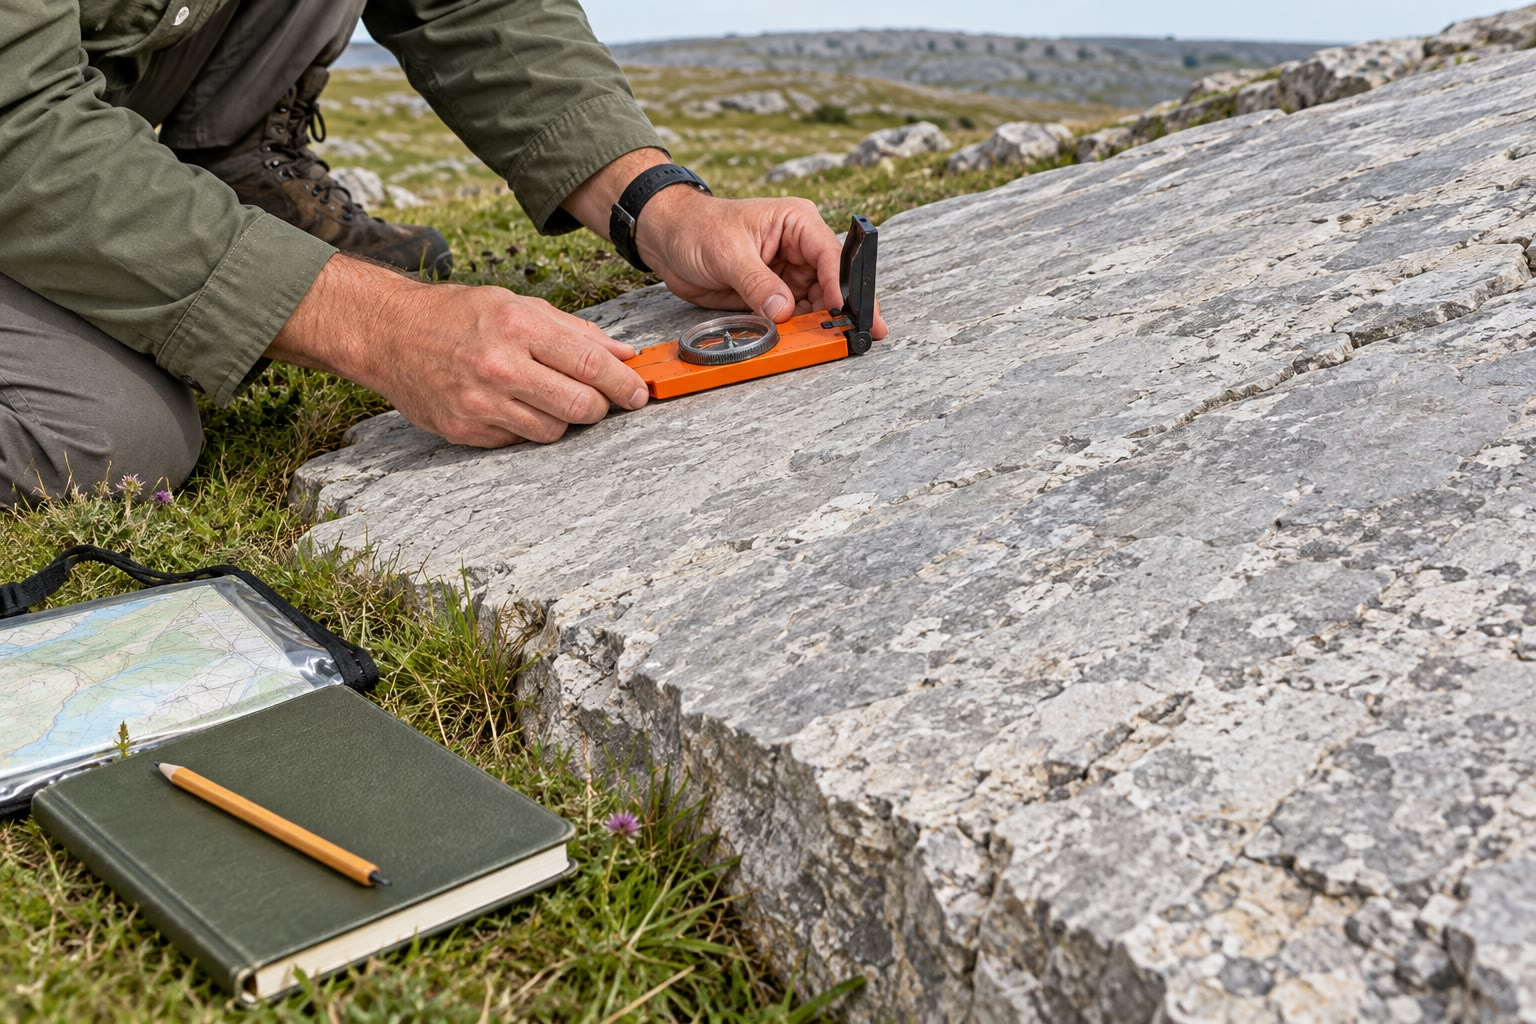
\includegraphics[width=0.6\linewidth]{images/book3/ai/b1-compass-clinometer.jpg}
\end{center}
\end{inthefield}

\begin{history}[De eerste geologische kaart van een land]
% ledger: gsl:smith-1815, commons:smith-1815
De landmeter William Smith, die kanalen groef en land droogmaakte in Engeland, merkte dat elke
gesteentelaag zijn eigen fossielen bevatte, in een volgorde die overal dezelfde was. Met de fossielen
om de lagen te herkennen, volgde hij ze meer dan vijftien jaar lang over het land. Zijn kaart,
\emph{A Delineation of the Strata of England and Wales, with part of
Scotland}, gedateerd 1 augustus 1815, geldt als de eerste \omterm{def:b1:geological-maps:geological-map}{geologische kaart} van een compleet land.
\begin{center}
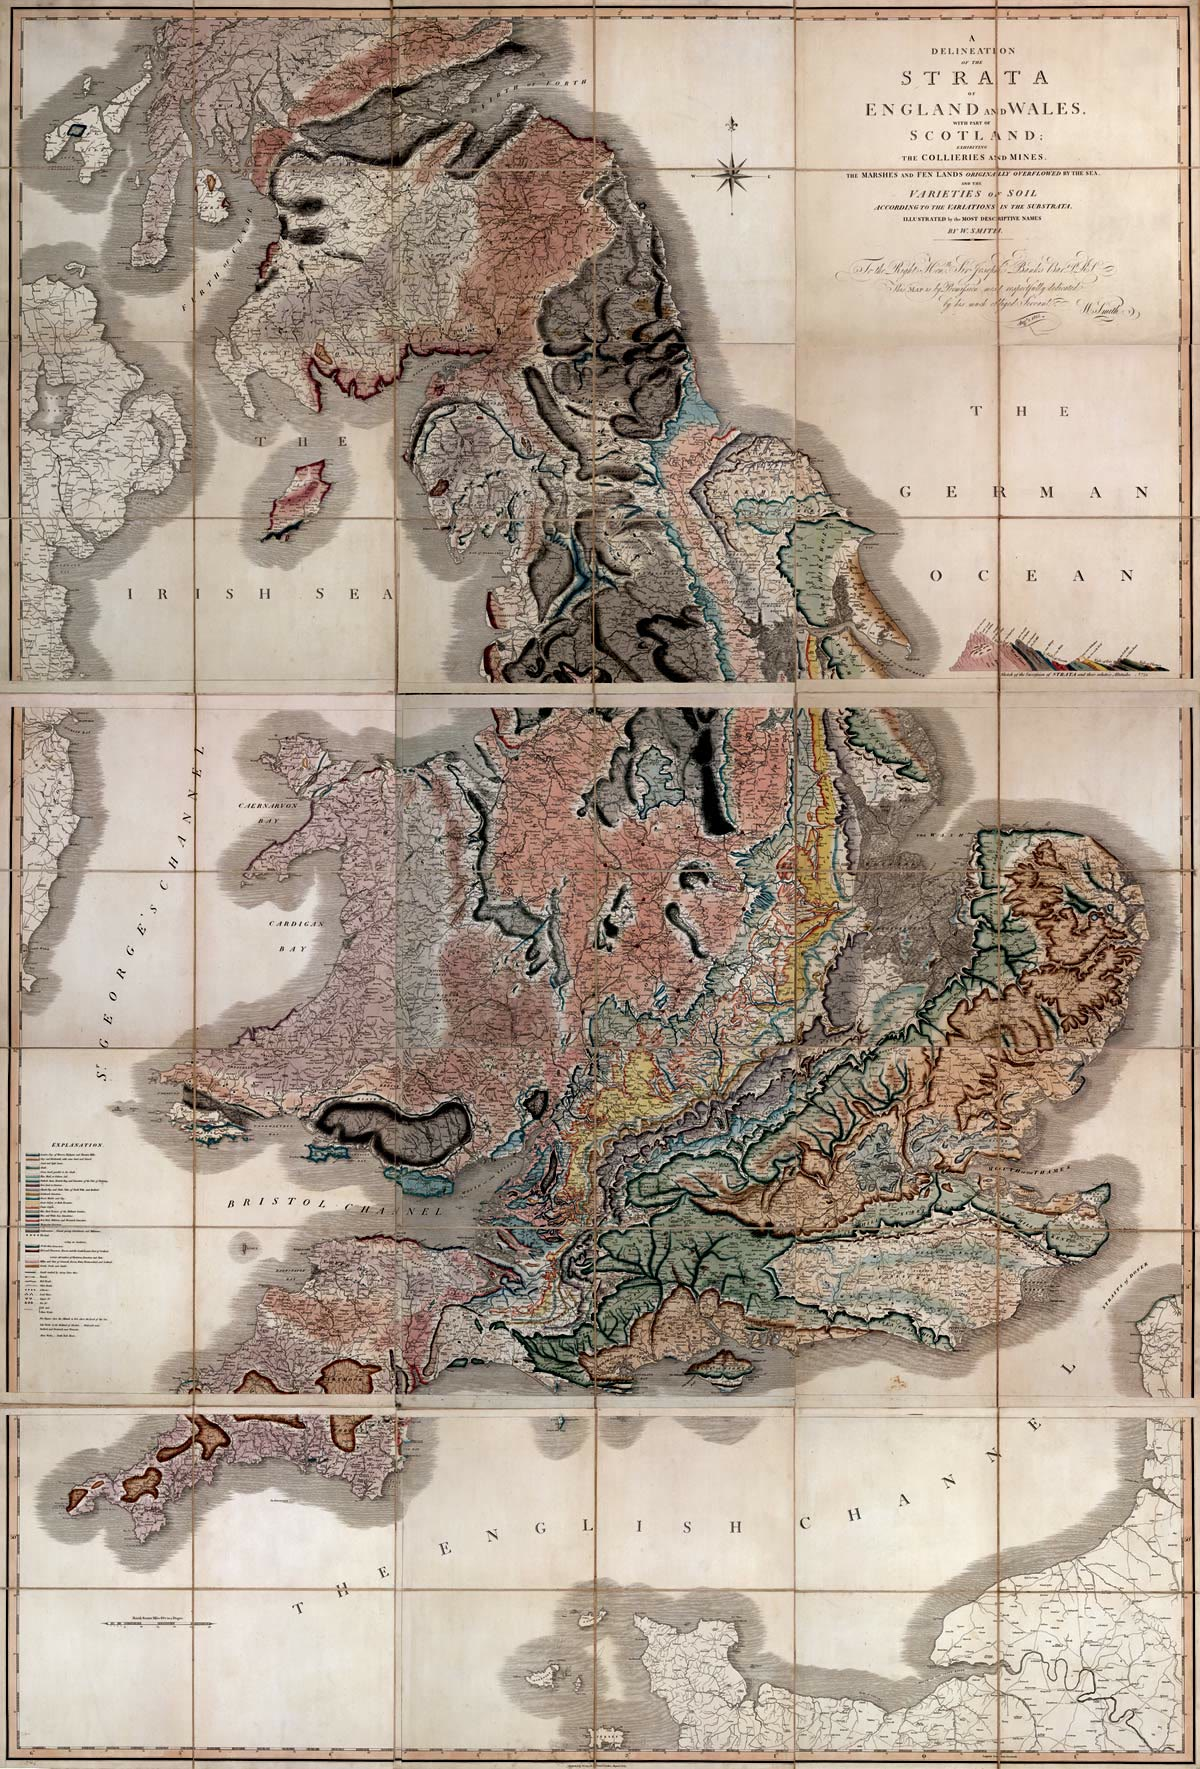
\includegraphics[width=0.36\linewidth]{images/book3/b1-smith-1815-map.jpg}

{\small William Smiths kaart van 1815 (publiek domein).}
\end{center}
\end{history}

\section{Oefeningen}

\begin{exercise}[$\star$]\label{exo:b1:geological-maps:1}
Definieer de \omterm{def:b1:geological-maps:attitude}{strijk}, de \omterm{def:b1:geological-maps:attitude}{helling} en de \omterm{def:b1:geological-maps:attitude}{hellingrichting} van een vlak. Een laag heeft de oriëntatie
$135/40$: geef haar \omterm{def:b1:geological-maps:attitude}{strijk} volgens de rechterhandregel en teken haar kaartsymbool.
\end{exercise}

\begin{exercise}[$\star$]\label{exo:b1:geological-maps:2}
Schrijf de vergelijking van het vlak met oriëntatie $090/30$ door het punt $(0, 0, 500)$, coördinaten
in meters. Op welke hoogte ligt het in $(1000, 0)$ en in $(0, 1000)$?
\end{exercise}

\begin{exercise}[$\star$]\label{exo:b1:geological-maps:3}
Op een kaart volgt het spoor van een contact precies de hoogtelijn \qty{350}{m}, over enkele kilometers
heuvels en dalen. Wat kan over het contact worden gezegd? En wat als zijn spoor een rechte lijn is over
heuvels en dalen heen?
\end{exercise}

\begin{exercise}[$\star$]\label{exo:b1:geological-maps:4}
Welke eenheid ontsluit zich op de kaart van de Varden Hills in de kern van de \omterm{def:b1:geological-maps:fold}{antiklinaal} langs de
rivier, en welke eenheid vormt de kern van de \omterm{def:b1:geological-maps:fold}{synklinaal}? Verklaar dat met het principe van superpositie.
\end{exercise}

\begin{exercise}[$\star\star$]\label{exo:b1:geological-maps:5}
Een contact wordt aangetroffen op hoogten van $\qty{300}{m}$ op $(0, 0)$, $\qty{300}{m}$ op $(1000, 0)$ en
$\qty{200}{m}$ op $(0, 500)$ (meter, $x$ naar het oosten, $y$ naar het noorden). Bepaal de \omterm{def:b1:geological-maps:attitude}{strijk}, de
\omterm{def:b1:geological-maps:attitude}{hellingrichting} en de \omterm{def:b1:geological-maps:attitude}{helling}, eerst door te redeneren met structuurlijnen, daarna met
\cref{thm:b1:geological-maps:three-point}.
\end{exercise}

\begin{exercise}[$\star\star$]\label{exo:b1:geological-maps:6}
Een valleibodem daalt noordwaarts met \qty{30}{m} per km. In welke richting wijst de V van de \omterm{def:b1:geological-maps:geological-map}{ontsluiting}
van een contact als het contact (a) horizontaal is; (b) \ang{20} naar het zuiden helt; (c) \ang{1} naar het
noorden helt; (d) \ang{20} naar het noorden helt? Motiveer met \cref{thm:b1:geological-maps:v-rule}.
\end{exercise}

\begin{exercise}[$\star\star$]\label{exo:b1:geological-maps:7}
In de situatie van de V-regel helt een contact stroomafwaarts met $a = 0.364$ (\ang{20}) en daalt de
valleibodem met $s = 0.03$. Een punt op de valleiwand ligt \qty{80}{m} hoger dan de bodem. Hoe ver
stroomopwaarts van de top ligt het spoor op dat punt?
\end{exercise}

\begin{exercise}[$\star\star$]\label{exo:b1:geological-maps:8}
De \omterm{def:b1:geological-maps:geological-map}{ontsluitingen} van de \omterm{def:b1:geological-maps:fold}{antiklinaal} van Varden sluiten zich rond het noordelijke uiteinde van zijn kern.
In welke richting helt de \omterm{def:b1:geological-maps:fold}{plooias}? Sluiten de \omterm{def:b1:geological-maps:geological-map}{ontsluitingen} van de \omterm{def:b1:geological-maps:fold}{synklinaal} zich naar het noorden of
naar het zuiden?
\end{exercise}

\begin{exercise}[$\star\star$]\label{exo:b1:geological-maps:9}
Aan welke kant van de breuk tonen de \omterm{def:b1:geological-maps:geological-map}{geologische kaart} en het oppervlak jongere eenheden? Welk blok is
omlaag bewogen? Controleer dat met het kaartsymbool.
\end{exercise}

\begin{exercise}[$\star\star\star$]\label{exo:b1:geological-maps:10}
Toon aan dat twee vlakken met oriëntaties $(\alpha_1, \delta_1)$ en $(\alpha_2, \delta_2)$ snijden langs een lijn
evenwijdig aan $\vec n_1 \times \vec n_2$, waarin $\vec n_i = (\tan\delta_i\sin\alpha_i,
\tan\delta_i\cos\alpha_i, 1)$. Pas het toe op de vlakken $090/30$ en $270/30$: welke lijn is het, en
wat voor \omterm{def:b1:geological-maps:fold}{plooi} vormen de twee vlakken?
\end{exercise}

\begin{exercise}[$\star\star\star$]\label{exo:b1:geological-maps:11}
Een verticale dijk strijkt \ang{045} en ontsluit zich in de oorsprong, op een valleibodem op hoogte
\qty{0}{m}. Waar kan haar spoor op een heuvel op \qty{300}{m} liggen? Een tweede dijk heeft dezelfde \omterm{def:b1:geological-maps:attitude}{strijk},
helt \ang{60} naar het zuidoosten en ontsluit zich ook in de oorsprong. Hoe ver van de oorsprong, en in
welke richting, ligt haar spoor op grond van \qty{300}{m}, gemeten loodrecht op de \omterm{def:b1:geological-maps:attitude}{strijk}?
\end{exercise}

\begin{exercise}[$\star\star\star$]\label{exo:b1:geological-maps:12}
In een \omterm{def:b1:geological-maps:dem}{digitaal hoogtemodel} met een raster van \qty{100}{m} ligt de grond op $(x, y)$ en op
$(x + 100, y)$ op 420 en \qty{405}{m}, en op $(x, y + 100)$ op \qty{412}{m}. Reken de grond in die cel
als een vlak: bereken de \omterm{def:b1:geological-maps:attitude}{helling} (in graden) en het \omterm{def:b1:spherical-astronomy:horizontal}{azimut} waarheen het vlak helt (de neerwaartse richting).
\end{exercise}

\section{Probleem: De Varden Hills oplossen}

\begin{problem}[{Weekendprobleem --- van boringen en een kaart naar de plooias, de breuk en de
geschiedenis van een streek}]
\label{pb:b1:geological-maps:1}
% all data computed in figdata/bachelor-1/varden_maps.py from the region's
% model (figdata/shared/region.py); invented region: exercise data, no ledger
Een bedrijf dat in de Varden Hills naar water boort, noteert op welke diepte zijn boringen de basis van de
kalksteen treffen; zijn geologen bepalen ook waar de breuk het terrein kruist. Coördinaten zijn in meters
oostwaarts en noordwaarts vanaf de zuidwestelijke hoek van de kaart; hoogten in meters boven zeeniveau.
Deel I gebruikt de gekleurde \omterm{def:b1:geological-maps:geological-map}{geologische kaart} van \cref{sec:b1:geological-maps:cut}.

\medskip
\noindent\textbf{Deel I --- De kaart lezen.}
\begin{enumerate}
  \item Noem de eenheden van de streek, van de oudste naar de jongste.
  \item Welke eenheden snijdt de rivier door, van west naar oost?
  \item Welke eenheid vormt de kern van de \omterm{def:b1:geological-maps:fold}{plooi} nabij $x = \qty{3.5}{km}$?
        Wat voor \omterm{def:b1:geological-maps:fold}{plooi} is dat?
  \item Welke eenheid vormt de kern van de \omterm{def:b1:geological-maps:fold}{plooi} nabij $x = \qty{7.5}{km}$?
        Wat voor \omterm{def:b1:geological-maps:fold}{plooi} is dat?
  \item Waarom zijn de schist en de graniet alleen dicht bij de rivier zichtbaar, in de kern van de
        eerste \omterm{def:b1:geological-maps:fold}{plooi}?
  \item Wat voor contact scheidt de zandsteen van de graniet? Motiveer met de kaart.
\end{enumerate}

\medskip
\noindent De boringen (diepte $d$ tot de basis van de kalksteen, grondhoogte $z_g$) en de drie punten
F1--F3 waar de breuk de bovenkant van het vaste gesteente kruist (F2, in de vallei, ligt onder het dunne
alluvium, dat de breuk niet doorsnijdt):

\begin{omfigure}
\begin{minipage}[c]{0.42\linewidth}
\centering\small
\begin{tabular}{lrrrr}
\hline
 & oost & noord & $z_g$ & $d$ \\
\hline
E1 & 4000 & 6000 & 435 & 261 \\
E2 & 4600 & 7200 & 432 & 428 \\
E3 & 5100 & 6400 & 512 & 586 \\
W1 & 1500 & 6000 & 524 & 669 \\
W2 & 2200 & 7200 & 421 & 459 \\
W3 & 2600 & 5400 & 319 & 209 \\
\hline
 & oost & noord & $z_g$ & \\
\hline
F1 & 4197 & 1000 & 405 & \\
F2 & 5824 & 3500 & 129 & \\
F3 & 7321 & 6500 & 482 & \\
\hline
\end{tabular}
\end{minipage}\hfill
\begin{minipage}[c]{0.56\linewidth}
\centering
\begin{tikzpicture}
\begin{axis}[axis equal image, xmin=0, xmax=10, ymin=0, ymax=8, width=\linewidth,
  tick label style={font=\scriptsize}, xlabel={oost (km)}, ylabel={noord (km)},
  label style={font=\footnotesize}]
\addplot[fill=black!8, draw=black!50, line width=0.3pt, even odd rule] table {figdata/out/shared-region-unit-schist.dat};
\addplot[fill=black!8, draw=black!50, line width=0.3pt, even odd rule] table {figdata/out/shared-region-unit-granite.dat};
\addplot[fill=icsTriassic!20, draw=black!50, line width=0.3pt, even odd rule] table {figdata/out/shared-region-unit-sandstone.dat};
\addplot[fill=icsJurassic!25, draw=black!50, line width=0.3pt, even odd rule] table {figdata/out/shared-region-unit-limestone.dat};
\addplot[fill=icsJurassic!8, draw=black!50, line width=0.3pt, even odd rule] table {figdata/out/shared-region-unit-shale.dat};
\addplot[fill=icsCretaceous!20, draw=black!50, line width=0.3pt, even odd rule] table {figdata/out/shared-region-unit-chalk.dat};
\addplot[fault] table {figdata/out/shared-region-fault.dat};
\addplot[fill=omLithAlluv, draw=black!50, line width=0.3pt, even odd rule] table {figdata/out/shared-region-unit-alluvium.dat};
\addplot[river] table {figdata/out/shared-region-river.dat};
\addplot[only marks, mark=*, mark size=1.6pt] table[x=x_km, y=y_km] {figdata/out/bachelor-1-varden_maps-boreholes.dat};
\addplot[only marks, mark=square*, mark size=1.5pt, omThm] table[x=x_km, y=y_km] {figdata/out/bachelor-1-varden_maps-fault.dat};
\begin{scope}[every node/.style={font=\scriptsize\bfseries, inner sep=1.5pt, fill=white, fill opacity=0.8, text opacity=1}]
  \node[above right] at (axis cs:4,6) {E1};
  \node[above] at (axis cs:4.6,7.2) {E2};
  \node[right] at (axis cs:5.1,6.4) {E3};
  \node[above left] at (axis cs:1.5,6) {W1};
  \node[above] at (axis cs:2.2,7.2) {W2};
  \node[left] at (axis cs:2.6,5.4) {W3};
  \node[left, text=omThm] at (axis cs:4.197,1) {F1};
  \node[left, text=omThm] at (axis cs:5.824,3.5) {F2};
  \node[left, text=omThm] at (axis cs:7.321,6.5) {F3};
\end{scope}
\end{axis}
\end{tikzpicture}
\end{minipage}
\end{omfigure}

\medskip
\noindent\textbf{Deel II --- De oostflank.}
\begin{enumerate}[resume]
  \item Bereken de hoogte van de basis van de kalksteen in E1, E2 en E3.
  \item Schrijf de vectoren $\overrightarrow{E_1E_2}$ en
        $\overrightarrow{E_1E_3}$.
  \item Bereken hun uitwendig product en oriënteer het naar boven.
  \item Leid hieruit de \omterm{def:b1:geological-maps:attitude}{helling} van de basis van de kalksteen op de oostflank af.
  \item Leid daaruit de \omterm{def:b1:geological-maps:attitude}{hellingrichting} af, en dan de \omterm{def:b1:geological-maps:attitude}{strijk} volgens de rechterhandregel.
  \item Is het resultaat in overeenstemming met het strijk- en hellingsymbool van de oostflank op de kaart?
\end{enumerate}

\medskip
\noindent\textbf{Deel III --- De plooi.}
\begin{enumerate}[resume]
  \item Bereken de hoogten van de basis van de kalksteen in W1, W2 en W3.
  \item Bereken een opwaartse normaal $\vec n_W$ op de basis van de kalksteen op de westflank.
  \item Leid hieruit de oriëntatie van de westflank af.
  \item Bereken een richting van het snijpunt van de twee flanken, de \omterm{def:b1:geological-maps:fold}{plooias}, als $\vec n_E \times \vec n_W$
        (met $\vec n_E$ uit vraag 9).
  \item Geef de richting (het \omterm{def:b1:spherical-astronomy:horizontal}{azimut} van de horizontale projectie van de as, in neerwaartse zin) en de
        \omterm{def:b1:geological-maps:attitude}{helling} (de hoek onder de horizontale) van de \omterm{def:b1:geological-maps:fold}{plooias}.
  \item De basis van de zandsteen ligt op de as op \qty{230}{m} waar de rivier hem kruist, nabij
        $y = \qty{4}{km}$. Hoeveel lager ligt hij op de as \qty{8}{km} verder naar het noorden? Is dit in
        overeenstemming met vraag 3 van deel I en met de sluiting van de \omterm{def:b1:geological-maps:geological-map}{ontsluitingen}?
\end{enumerate}

\medskip
\noindent\textbf{Deel IV --- De breuk en de geschiedenis.}
\begin{enumerate}[resume]
  \item Bereken uit F1, F2 en F3 de oriëntatie van de breuk.
  \item Langs de breuk zijn de eenheden aan het oppervlak aan de oost-zuidoostkant jonger dan die er
        tegenover liggen. Welk blok is omlaag bewogen? Is de breuk normaal of omgekeerd?
  \item De rechte lijn van F1 naar F3 gaat ongeveer \qty{200}{m} west van F2 voorbij. Waarom buigt het
        spoor van de breuk naar het oost-zuidoosten waar het de rivierdal kruist, bij F2?
  \item Zet in volgorde: plooiing; afzetting van het krijt; breukvorming; intrusie van de graniet;
        erosie vóór de zandsteen; afzetting van het alluvium.
  \item Het krijt is 90 miljoen jaar oud en is geplooid; het alluvium is in de laatste 2.58 miljoen jaar
        afgezet en is niet gebroken. Tussen welke leeftijden hebben de plooiing en de breukvorming
        plaatsgevonden?
  \item Om de breuk op \qty{1000}{m} onder zeeniveau onder F1 te bereiken, hoe ver van F1 en in welke
        richting moet een verticale put worden geboord?
\end{enumerate}
\end{problem}
